\chapter{Resultados}\label{cap:Resultados}

Este capítulo apresenta os experimentos realizados com a implementação do algoritmo \textit{LZ77} desenvolvida na biblioteca \textit{Komm}, bem como comparações com outras implementações externas do mesmo método.  
Os demais algoritmos disponíveis na \textit{Komm} (Huffman, Shannon--Fano, LZ78 e LZW) foram utilizados apenas como referência para fins de contextualização dos resultados.

\section{Conjuntos de dados e protocolo experimental}

Foram utilizados dois tipos de arquivos: (i) \textbf{textos} e (ii) \textbf{imagens}.  
O texto escolhido foi o livro \textit{Alice’s Adventures in Wonderland}, do Projeto Gutenberg\footnote{\url{https://www.gutenberg.org/ebooks/11}}, por se tratar de um corpus literário clássico amplamente utilizado em experimentos de compressão sem perdas.  
O arquivo possui tamanho de 154.573 bytes e apresenta ampla variedade de caracteres e repetições, sendo adequado para testar diferentes tamanhos de janela no \textit{LZ77}.  

As imagens utilizadas foram bitmaps (\textbf{BMP}) simples, escolhidas por possuírem regiões de baixa entropia e padrões espaciais redundantes, que permitem observar o comportamento do algoritmo em fontes bidimensionais.  
A Figura~\ref{fig:smiley} mostra a imagem \textit{smiley} (246~bytes) e a Figura~\ref{fig:snail} a imagem \textit{snail} (196.666~bytes).

\begin{figure}[h]
  \centering
  \caption{Imagem bitmap (BMP) \textit{smiley}.}
  \label{fig:smiley}
  
\includegraphics[width=5cm]{figuras/smiley-large.png}
  \fonte{Adaptada de \url{https://cse1.net/recaps/graphics}.}
\end{figure}

\begin{figure}[h]
  \centering
  \caption{Imagem bitmap (BMP) \textit{snail}.}
  \label{fig:snail}
  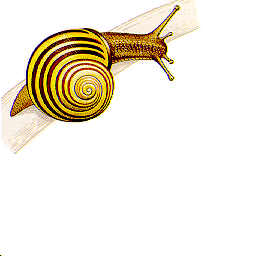
\includegraphics[width=5cm]{figuras/snail.png}
  \fonte{Adaptada de \url{https://people.math.sc.edu/Burkardt/data/bmp/bmp.html}.}
\end{figure}

\pagebreak
\section{Métricas de avaliação}

As seguintes métricas foram utilizadas para avaliar o desempenho dos algoritmos:
\begin{itemize}
  \item \textbf{Taxa de compressão}: relação entre o tamanho comprimido e o tamanho original (quanto menor, melhor).
  \item \textbf{Tempo de compressão e descompressão}: medido em segundos.
  \item \textbf{Memória pico}: quantidade máxima de memória alocada durante a execução (em MB).
  \item \textbf{Integridade}: verificação de \emph{round trip}, isto é, \texttt{decode(encode(x)) == x}.
\end{itemize}

\section{Resultados do LZ77 na \textit{Komm}}

Foram consideradas duas implementações populares: \textbf{FastLZ}\footnote{https://github.com/ariya/FastLZ} (C) e \textbf{LZ77-Compressor}\footnote{https://github.com/ariya/FastLZ} (Python). As configurações efetivas foram: \(W=8\,\text{KiB}\) e \(L=264\) bytes no \textit{FastLZ}; no \textit{LZ77-Compressor}, \(W\) variou entre 100 e 400 bytes e \(L=15\) bytes. Na \textit{Komm}, \(W\) e \(L\) são parametrizáveis; para comparação, utilizaram-se configurações próximas às disponíveis nas bibliotecas externas quando pertinente, além de uma configuração de referência com \(W=64\,\text{kB}\).

\begin{figure}[htp]
  \centering
  \caption{Texto \textit{Alice}: taxa de compressão (menor é melhor).}
  \label{fig:komm-alice-compression}
  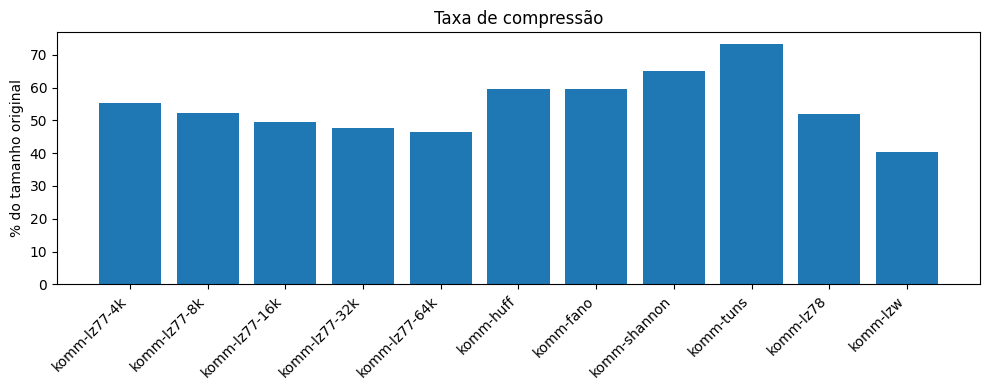
\includegraphics[width=15cm]{figuras/komm_alice_compression.png}
  \fonte{Elaborada pelo autor.}
\end{figure}

\begin{figure}[htp]
  \centering
  \caption{Texto \textit{Alice}: memória pico.}
  \label{fig:komm-alice-memory}
  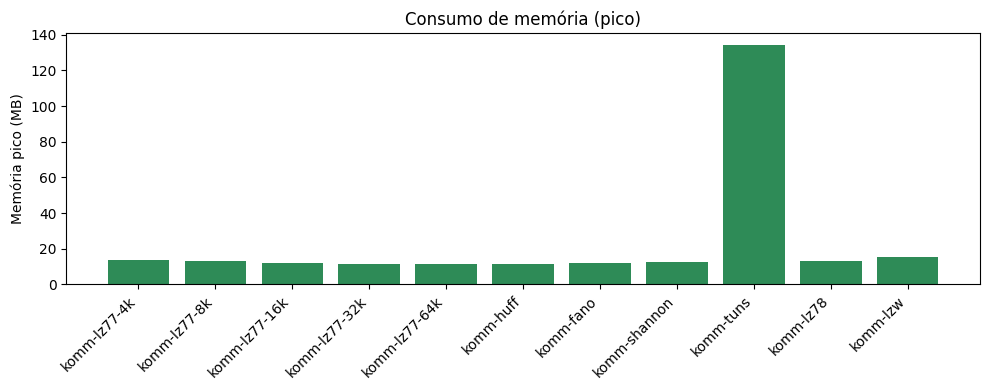
\includegraphics[width=15cm]{figuras/komm_alice_memory.png}
  \fonte{Elaborada pelo autor.}
\end{figure}

\begin{figure}[htp]
  \centering
  \caption{Texto \textit{Alice}: tempo de compressão.}
  \label{fig:komm-alice-time}
  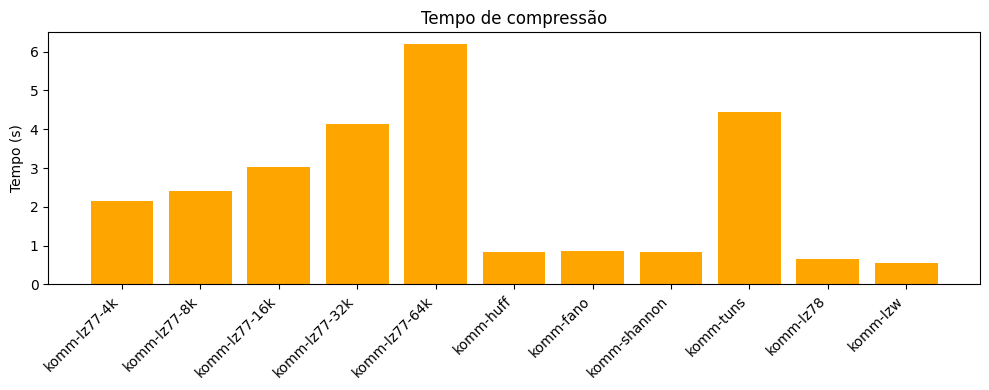
\includegraphics[width=15cm]{figuras/komm_alice_time.png}
  \fonte{Elaborada pelo autor.}
\end{figure}

\noindent\textbf{Análise (texto):}
\begin{itemize}
  \item O \textit{LZ77} apresentou o \emph{trade-off} esperado: janelas maiores proporcionam melhor compressão, mas aumentam o tempo e o consumo de memória.
  \item Para o arquivo \textit{Alice}, o ganho de compressão é significativo ao aumentar \(W\) de 400~B para 32~kB, estabilizando a partir de 64~kB.
  \item Em comparação, Huffman e Shannon--Fano mantêm desempenho rápido e baixo uso de memória, porém com taxas de compressão inferiores.
\end{itemize}

\begin{figure}[htp]
  \centering
  \caption{Imagem \textit{smiley}: taxa de compressão (menor é melhor).}
  \label{fig:komm-smiley-compression}
  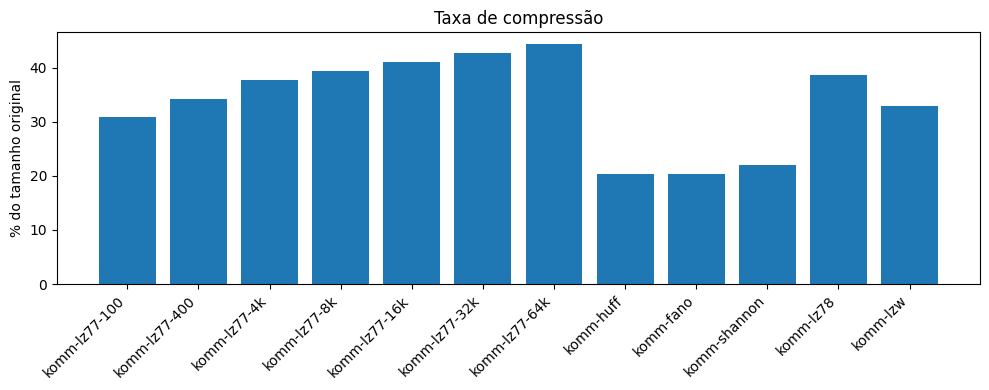
\includegraphics[width=15cm]{figuras/komm_smiley_compression.png}
  \fonte{Elaborada pelo autor.}
\end{figure}

\begin{figure}[htp]
  \centering
  \caption{Imagem \textit{smiley}: memória pico.}
  \label{fig:komm-smiley-memory}
  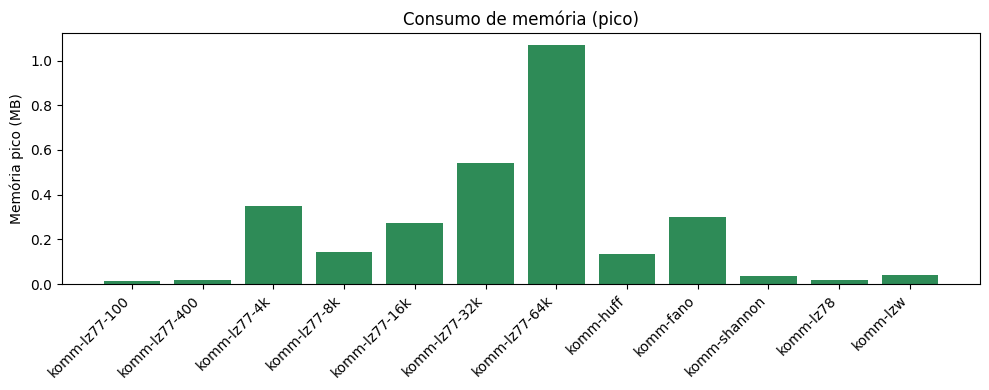
\includegraphics[width=15cm]{figuras/komm_smiley_memory.png}
  \fonte{Elaborada pelo autor.}
\end{figure}

\begin{figure}[htp]
  \centering
  \caption{Imagem \textit{smiley}: tempo de compressão.}
  \label{fig:komm-smiley-time}
  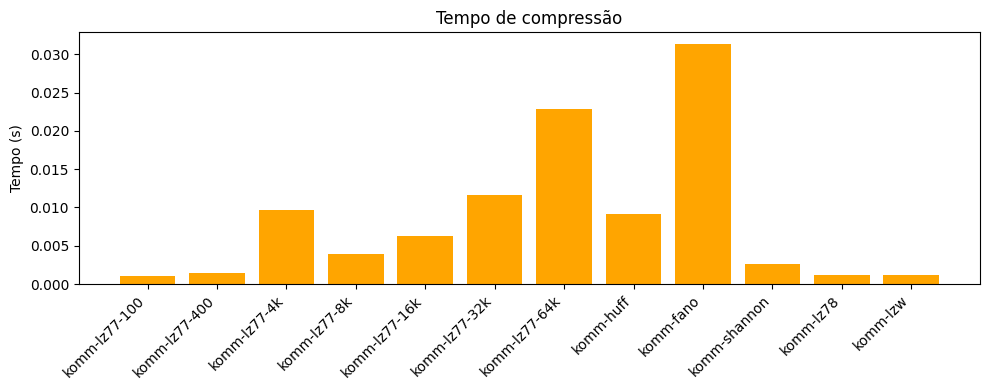
\includegraphics[width=15cm]{figuras/komm_smiley_time.png}
  \fonte{Elaborada pelo autor.}
\end{figure}

\begin{figure}[htp]
  \centering
  \caption{Imagem \textit{snail}: taxa de compressão (menor é melhor).}
  \label{fig:komm-snail-compression}
  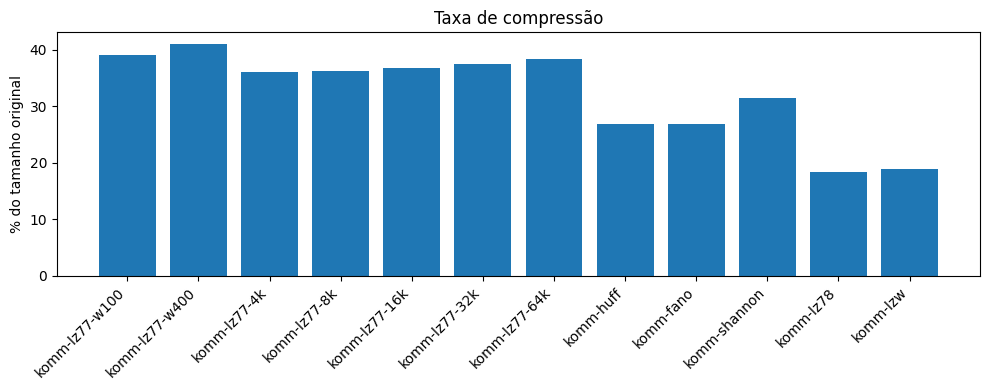
\includegraphics[width=15cm]{figuras/komm_snail_compression.png}
  \fonte{Elaborada pelo autor.}
\end{figure}

\begin{figure}[htp]
  \centering
  \caption{Imagem \textit{snail}: memória pico.}
  \label{fig:komm-snail-memory}
  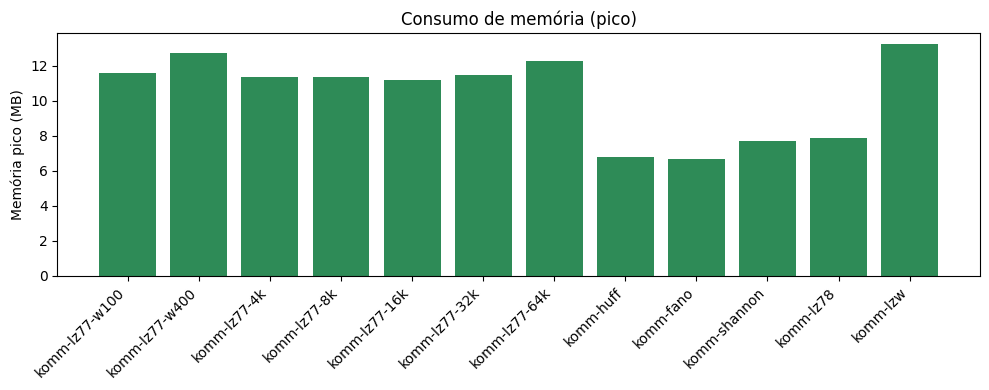
\includegraphics[width=15cm]{figuras/komm_snail_memory.png}
  \fonte{Elaborada pelo autor.}
\end{figure}

\begin{figure}[htp]
  \centering
  \caption{Imagem \textit{snail}: tempo de compressão.}
  \label{fig:komm-snail-time}
  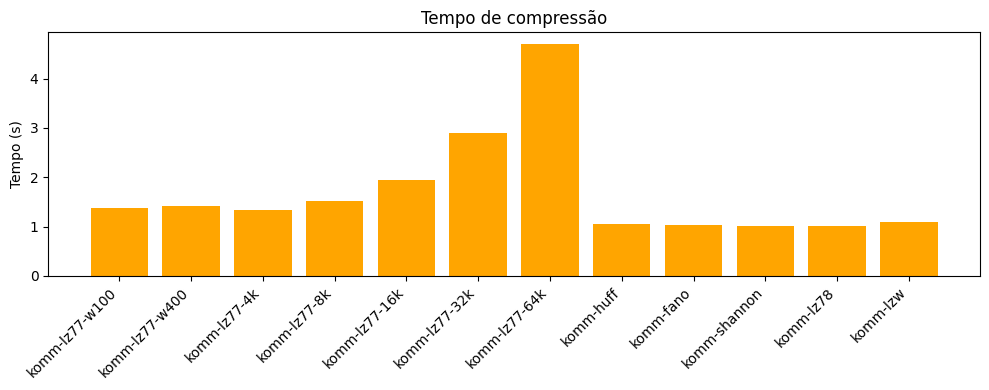
\includegraphics[width=15cm]{figuras/komm_snail_time.png}
  \fonte{Elaborada pelo autor.}
\end{figure}

\noindent\textbf{Análise (imagens):}
\begin{itemize}
  \item Nas imagens \textit{smiley} e \textit{snail}, o \textit{LZ77} apresentou menor ganho de compressão em comparação ao texto, o que é esperado dada a menor redundância sequencial.
  \item Janelas maiores continuam a reduzir ligeiramente a taxa de compressão, porém com crescimento do custo computacional.
  \item A relação entre tempo e memória manteve comportamento aproximadamente linear com o tamanho da janela.
\end{itemize}

\begin{quadro}[ht]
\caption{Resumo de tempo e memória na compressão da imagem \textit{smiley} (implementações na \textit{Komm}).}
\label{quadro:resultados-komm-smiley}
\begin{tabular}{|l|r|r|}
    \hline
    \textbf{Algoritmo} & \textbf{Tempo (s)} & \textbf{Memória pico (MB)} \\ \hline
    komm-lz77-100   & 1,382 & 12,128  \\ \hline
    komm-lz77-400   & 1,416 & 13,330  \\ \hline
    komm-lz77-8k   & 0,0039 & 148,218  \\ \hline
    komm-lz77-16k  & 0,0062 & 287,370  \\ \hline
    komm-lz77-32k  & 0,0115 & 566,106  \\ \hline
    komm-lz77-64k  & 0,0228 & 112,295  \\ \hline
    komm-huff      & 0,0092 & 140,961  \\ \hline
    komm-fano      & 0,0313 & 314,210  \\ \hline
    komm-shannon   & 0,0026 & 38,195   \\ \hline
    komm-lz78      & 0,0011 & 19,928   \\ \hline
    komm-lzw       & 0,0011 & 43,084   \\ \hline
\end{tabular}
\fonte{Elaborada pelo autor.}
\end{quadro}

\section{Comparação com implementações externas de LZ77}\label{sec:externas}

Foram consideradas duas implementações populares do algoritmo \textit{LZ77}: \textbf{FastLZ}\footnote{\url{https://github.com/ariya/FastLZ}} (em C) e \textbf{LZ77-Compressor}\footnote{\url{https://github.com/manassra/LZ77-Compressor}} (em Python).  
As configurações padrão dessas bibliotecas são:
\begin{itemize}
  \item \textbf{FastLZ}: janela de 8~kB e \textit{lookahead} de 264~bytes;
  \item \textbf{LZ77-Compressor}: janela variável (100–400~bytes) e \textit{lookahead} fixo de 15~bytes.
\end{itemize}

Na \textit{Komm}, foi possível parametrizar \(W\) e \(L\) livremente, permitindo a replicação aproximada das condições dessas bibliotecas, além de uma configuração de referência com \(W=64\,\text{kB}\).

\begin{figure}[htp]
  \centering
  \caption{Texto \textit{Alice}: taxa de compressão (menor é melhor).}
  \label{fig:external-alice-compression}
  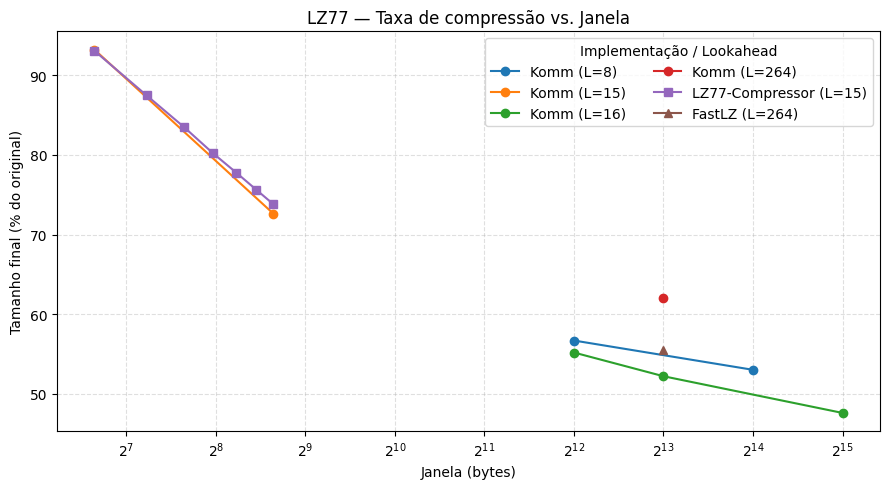
\includegraphics[width=15cm]{figuras/lz77_alice_compression_window.png}
  \fonte{Elaborada pelo autor.}
\end{figure}

\begin{figure}[htp]
  \centering
  \caption{Texto \textit{Alice}: memória pico.}
  \label{fig:external-alice-memory}
  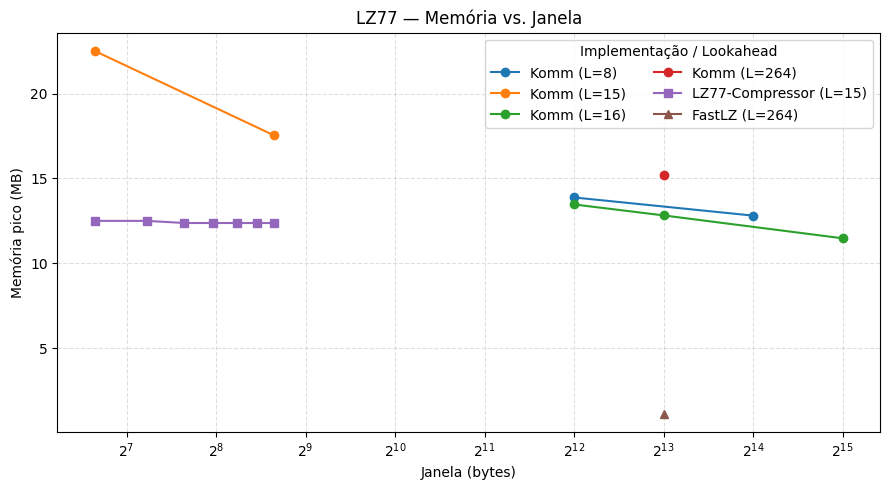
\includegraphics[width=15cm]{figuras/lz77_alice_memory_window.png}
  \fonte{Elaborada pelo autor.}
\end{figure}

\begin{figure}[htp]
  \centering
  \caption{Texto \textit{Alice}: tempo de compressão.}
  \label{fig:external-alice-time}
  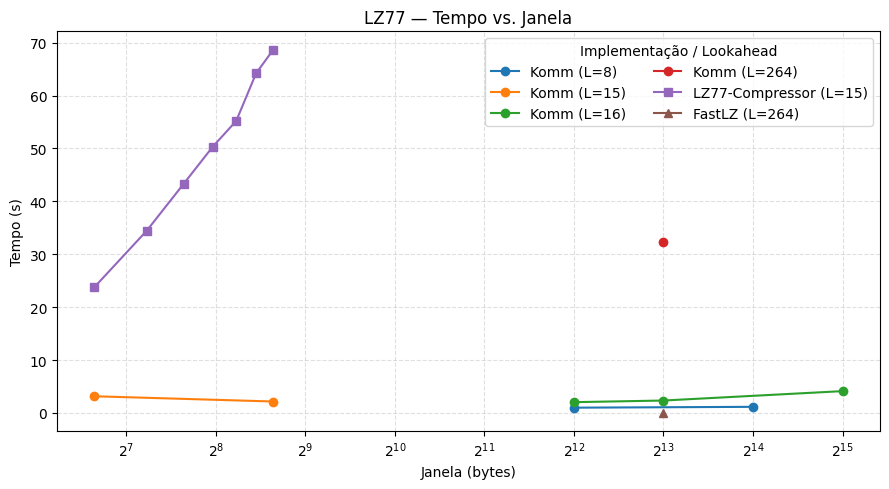
\includegraphics[width=15cm]{figuras/lz77_alice_time_window.png}
  \fonte{Elaborada pelo autor.}
\end{figure}

\noindent\textbf{Análise (texto):}
\begin{itemize}
  \item A implementação \textit{FastLZ} apresentou tempos de compressão inferiores, resultado coerente com sua implementação em C voltada à velocidade.
  \item A versão da \textit{Komm}, com \(W=64\,\text{kB}\), obteve taxas de compressão próximas, mostrando boa eficiência mesmo em Python.
  \item A biblioteca \textit{LZ77-Compressor} apresentou maior tempo de execução, mas consumo de memória reduzido.
\end{itemize}

\begin{figure}[htp]
  \centering
  \caption{Imagem \textit{smiley}: taxa de compressão (menor é melhor).}
  \label{fig:external-smiley-compression}
  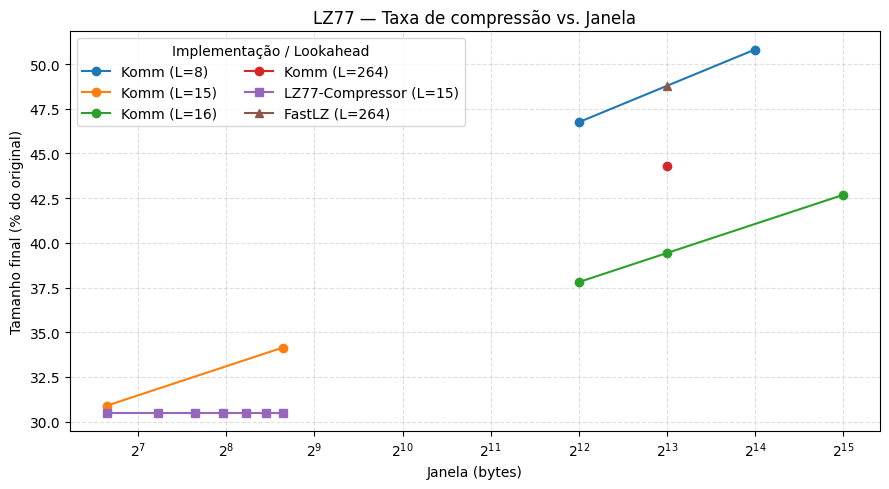
\includegraphics[width=15cm]{figuras/lz77_smiley_compression_window.png}
  \fonte{Elaborada pelo autor.}
\end{figure}

\begin{figure}[htp]
  \centering
  \caption{Imagem \textit{smiley}: memória pico.}
  \label{fig:external-smiley-memory}
  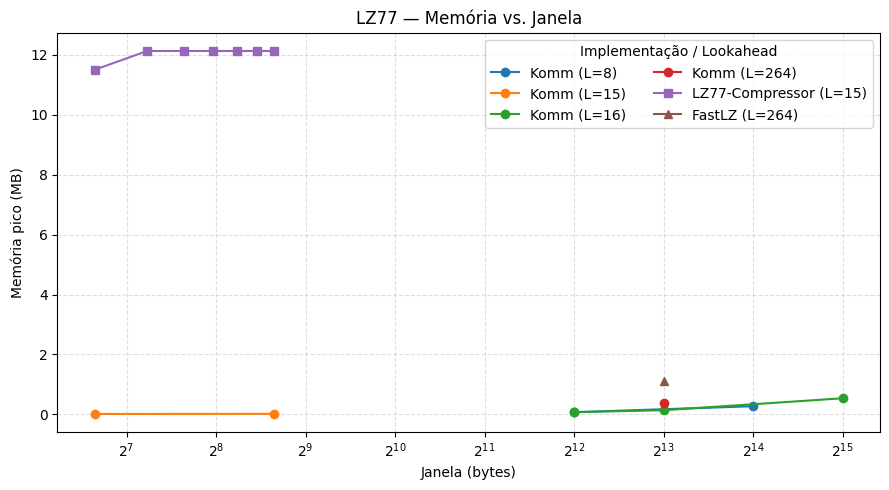
\includegraphics[width=15cm]{figuras/lz77_smiley_memory_window.png}
  \fonte{Elaborada pelo autor.}
\end{figure}

\begin{figure}[htp]
  \centering
  \caption{Imagem \textit{smiley}: tempo de compressão.}
  \label{fig:external-smiley-time}
  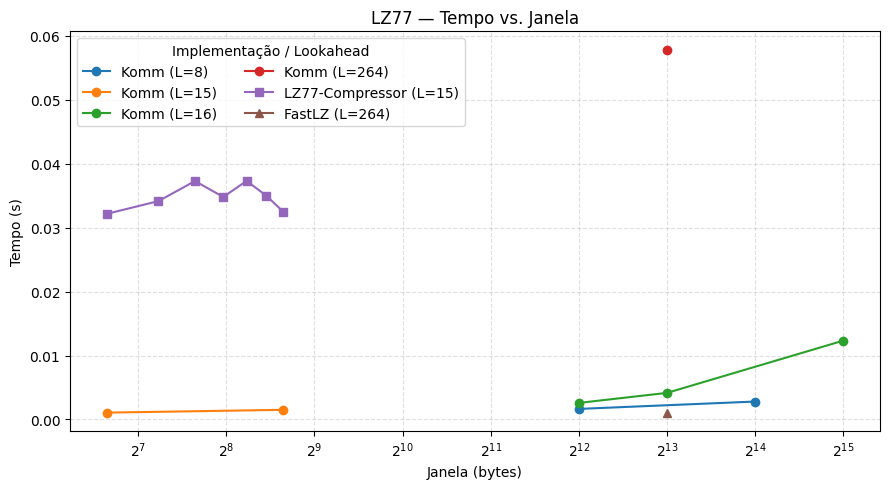
\includegraphics[width=15cm]{figuras/lz77_smiley_time_window.png}
  \fonte{Elaborada pelo autor.}
\end{figure}

\noindent\textbf{Análise (imagens):}
\begin{itemize}
  \item A implementação da \textit{Komm} superou as versões externas em taxa de compressão, principalmente para janelas maiores.
  \item O \textit{FastLZ} manteve vantagem em tempo de execução, mas com menor eficiência de compressão.
  \item O \textit{LZ77-Compressor} exibiu desempenho inferior em tempo e memória, refletindo limitações inerentes à implementação em Python puro.
\end{itemize}

\section{Discussão}

Os resultados obtidos confirmam o comportamento clássico do \textit{LZ77}:  
(i) janelas maiores aumentam a capacidade de reutilização de padrões, melhorando a taxa de compressão;  
(ii) esse ganho é acompanhado de aumento linear de tempo e memória;  
(iii) implementações em linguagens compiladas, como C, tendem a dominar em desempenho absoluto.  

Apesar disso, a versão implementada na \textit{Komm} mostrou-se competitiva, validando a adequação da arquitetura modular proposta e seu potencial como ferramenta educacional e de pesquisa.  
Todos os testes preservaram a integridade dos dados (\emph{round trip} verdadeiro).
